\documentclass[11pt, letterpaper]{article}

\usepackage[margin=1in]{geometry}
\usepackage{graphicx}
\usepackage{amsmath, amssymb}
\usepackage{booktabs}
\usepackage{hyperref}
\usepackage{listings}
\usepackage{xcolor}
\usepackage{float}
\usepackage{caption}
\usepackage{subcaption}
\usepackage[backend=biber, style=numeric, sorting=none]{biblatex}
\addbibresource{references.bib}

\hypersetup{
    colorlinks=true,
    linkcolor=blue!60!black,
    citecolor=blue!60!black,
    urlcolor=blue!60!black,
}

\lstset{
    language=Python,
    basicstyle=\ttfamily\small,
    keywordstyle=\color{blue!70!black},
    stringstyle=\color{red!60!black},
    commentstyle=\color{green!50!black}\itshape,
    numbers=left,
    numberstyle=\tiny\color{gray},
    frame=single,
    breaklines=true,
    captionpos=b,
}

\title{%
    \textbf{Teaching a Tiny Non-Transformer Model Arithmetic Reasoning via Reinforcement Learning} \\[0.5em]
    \large GRPO Fine-Tuning of LFM2-350M for Mathematical Expression Generation
}
\author{Wes Griffin \\ Ransom Everglades School \\ Advanced Machine Learning}
\date{April 2026}

\begin{document}

\maketitle

\begin{abstract}
This project explores whether reinforcement learning can teach a small (350M parameter) non-transformer language model to generate valid mathematical expressions that evaluate to target numbers. Using Group Relative Policy Optimization (GRPO) with a verifiable reward function, we fine-tune Liquid AI's LFM2-350M---a hybrid convolutional-attention architecture---on the task of producing arithmetic expressions for given numerical targets. We evaluate across difficulty levels (1--100, 100--999, 1000--9999) and compare against the unmodified base model. Our results demonstrate that RL with verifiable rewards can induce structured arithmetic reasoning in small, novel-architecture language models, with implications for efficient on-device AI deployment.
\end{abstract}

% ============================================================================
\section{Introduction}
\label{sec:intro}

Large language models (LLMs) have demonstrated remarkable capabilities in mathematical reasoning, with models like DeepSeek-R1 and OpenAI's o1 achieving near-human performance on competition-level problems \cite{deepseekmath}. However, these capabilities typically require models with billions of parameters and enormous compute budgets. A natural question arises: \emph{can reinforcement learning induce structured reasoning in much smaller models?}

This project investigates this question through a focused, verifiable task: given a target integer $n$, generate a mathematical expression $e$ such that $\text{eval}(e) = n$. For example, given the target 73, valid responses include \texttt{70 + 3}, \texttt{146 / 2}, or \texttt{9 * 8 + 1}. This task is ideal for RL because:

\begin{enumerate}
    \item The reward is \textbf{perfectly verifiable}---we can programmatically check if $\text{eval}(e) = n$.
    \item The task requires \textbf{compositional reasoning}---the model must understand how arithmetic operations compose.
    \item Multiple valid solutions exist, encouraging \textbf{expression diversity}.
    \item Difficulty scales naturally with the magnitude of $n$.
\end{enumerate}

We choose Liquid AI's LFM2-350M \cite{lfm2} as our base model for several reasons. First, at 354M parameters, it is small enough to train on modest hardware. Second, it uses a novel hybrid architecture combining gated short-range convolutions with grouped query attention, making it architecturally distinct from the transformer-only models typically used in RL fine-tuning research. Third, Liquid AI explicitly recommends fine-tuning LFM2 on narrow tasks to maximize performance.

Our training method is Group Relative Policy Optimization (GRPO) \cite{deepseekmath}, implemented via Hugging Face's TRL library \cite{trl}. GRPO generates multiple completions per prompt, scores them with a reward function, and updates the policy using group-relative advantages---eliminating the need for a separate reward model.

% ============================================================================
\section{Data Exploration and Preparation}
\label{sec:data}

\subsection{Dataset Construction}

Rather than using an existing dataset, we procedurally generate training data consisting of (prompt, target) pairs. Each prompt asks the model to produce a math expression equaling the target number, formatted with \texttt{<expr></expr>} tags.

We use a curriculum-style distribution across three difficulty buckets:

\begin{table}[H]
\centering
\caption{Training data distribution across difficulty levels.}
\label{tab:data-dist}
\begin{tabular}{lccc}
\toprule
\textbf{Difficulty} & \textbf{Range} & \textbf{Fraction} & \textbf{Count} \\
\midrule
Easy   & 1--100    & 40\% & 4,000 \\
Medium & 100--999  & 35\% & 3,500 \\
Hard   & 1,000--9,999 & 25\% & 2,500 \\
\bottomrule
\end{tabular}
\end{table}

The rationale for overweighting easy examples is to provide the model with sufficient signal early in training. Since the 350M model starts with minimal arithmetic ability, easy targets (where simple expressions like \texttt{50 + 7} suffice) generate more positive reward signal, allowing the policy gradient to learn basic expression structure before tackling harder targets.

\begin{figure}[H]
\centering
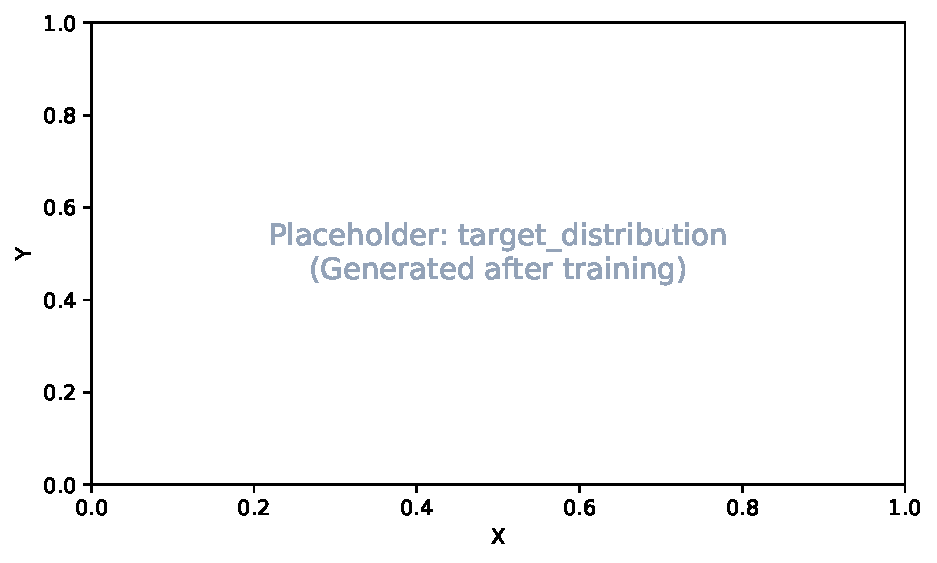
\includegraphics[width=0.75\textwidth]{figures/target_distribution.pdf}
\caption{Distribution of target numbers in the training set, colored by difficulty bucket.}
\label{fig:target-dist}
\end{figure}

\subsection{Prompt Format}

Each training example is formatted as a chat conversation:

\begin{lstlisting}[caption={Prompt format used during training.}]
System: You are a math assistant. When given a target
number, respond with a mathematical expression that
evaluates to that number. Use only integers, +, -, *,
/, and parentheses. Put your expression inside
<expr></expr> tags.

User: Find a math expression that equals 73.
Respond with ONLY <expr>YOUR_EXPRESSION</expr>.
\end{lstlisting}

The structured output format (\texttt{<expr>} tags) enables reliable extraction and evaluation. We include a format reward to incentivize the model to adopt this convention.

\subsection{Evaluation Set}

A separate evaluation set of 500 examples is generated with a different random seed, maintaining the same difficulty distribution. This ensures no target overlap between training and evaluation.

% ============================================================================
\section{Methodology}
\label{sec:method}

\subsection{Model Architecture}

LFM2-350M \cite{lfm2} is a hybrid model with 16 layers: 10 double-gated short-range LIV convolution blocks and 6 grouped query attention (GQA) blocks. Key specifications:

\begin{table}[H]
\centering
\caption{LFM2-350M architecture details.}
\begin{tabular}{ll}
\toprule
\textbf{Property} & \textbf{Value} \\
\midrule
Parameters & 354,483,968 \\
Layers & 16 (10 conv + 6 attn) \\
Context length & 32,768 tokens \\
Vocabulary size & 65,536 \\
Precision & bfloat16 \\
Pre-training data & 10 trillion tokens \\
\bottomrule
\end{tabular}
\end{table}

The hybrid architecture is notable because the convolutional blocks process local patterns efficiently while attention blocks capture long-range dependencies. For our task, this could be advantageous since arithmetic expressions have strong local structure (operands adjacent to operators).

\subsection{GRPO Algorithm}

Group Relative Policy Optimization \cite{deepseekmath} works as follows at each training step:

\begin{enumerate}
    \item \textbf{Generate}: Sample a batch of prompts; for each, generate $G$ completions $\{o_1, \ldots, o_G\}$.
    \item \textbf{Score}: Compute reward $r_i$ for each completion using the reward function.
    \item \textbf{Normalize}: Compute group-relative advantage:
    \[
        \hat{A}_{i,t} = \frac{r_i - \text{mean}(\mathbf{r})}{\text{std}(\mathbf{r})}
    \]
    \item \textbf{Update}: Minimize the clipped surrogate loss:
    \[
        \mathcal{L}_{\text{GRPO}}(\theta) = -\frac{1}{\sum_{i=1}^G |o_i|} \sum_{i=1}^G \sum_{t=1}^{|o_i|} \min\!\left( \rho_{i,t} \hat{A}_{i,t},\; \text{clip}(\rho_{i,t}, 1{-}\epsilon, 1{+}\epsilon) \hat{A}_{i,t} \right)
    \]
    where $\rho_{i,t} = \frac{\pi_\theta(o_{i,t} | q, o_{i,<t})}{\pi_{\theta_{\text{old}}}(o_{i,t} | q, o_{i,<t})}$.
\end{enumerate}

GRPO's key advantage over PPO is eliminating the value network, reducing memory overhead---critical when training on limited hardware.

\subsection{Reward Design}

We use a composite reward function with four components:

\begin{table}[H]
\centering
\caption{Reward function components and weights.}
\label{tab:rewards}
\begin{tabular}{llcl}
\toprule
\textbf{Component} & \textbf{Description} & \textbf{Weight} & \textbf{Range} \\
\midrule
Correctness & Binary: $\text{eval}(e) = n$ & 2.0 & $\{0, 1\}$ \\
Closeness & $\max(0, 1 - |r - n|/|n|)$ & 0.5 & $[0, 1]$ \\
Format & Uses \texttt{<expr>} tags & 0.3 & $\{0, 0.5\}$ \\
Complexity & Bonus for multiple operators & 0.2 & $[0, 0.3]$ \\
\bottomrule
\end{tabular}
\end{table}

The \textbf{correctness} reward dominates (weight 2.0) because exact evaluation is the primary objective. The \textbf{closeness} reward provides gradient signal even for incorrect answers---without it, early training would be extremely sparse since the base model rarely produces correct expressions. The \textbf{format} reward teaches output structure, and the \textbf{complexity} reward gently encourages expressions more interesting than trivial identity (e.g., \texttt{73} for target 73).

Expression evaluation uses a safe AST-based parser that only allows integer literals and basic arithmetic operators (\texttt{+}, \texttt{-}, \texttt{*}, \texttt{/}, \texttt{//}, \texttt{\%}, \texttt{**}), preventing code injection.

\subsection{Training Configuration}

\begin{table}[H]
\centering
\caption{Training hyperparameters.}
\label{tab:hyperparams}
\begin{tabular}{ll}
\toprule
\textbf{Parameter} & \textbf{Value} \\
\midrule
LoRA rank $r$ & 32 \\
LoRA alpha $\alpha$ & 64 \\
LoRA dropout & 0.05 \\
Target modules & \texttt{q,k,v,o\_proj}, \texttt{gate,up,down\_proj} \\
Learning rate & $5 \times 10^{-5}$ \\
LR scheduler & Cosine with 5\% warmup \\
Batch size & 4 per device \\
Gradient accumulation & 4 steps \\
Completions per prompt ($G$) & 8 \\
Max completion length & 128 tokens \\
Epochs & 3 \\
Precision & bfloat16 \\
\bottomrule
\end{tabular}
\end{table}

We use LoRA \cite{lora} (Low-Rank Adaptation) rather than full fine-tuning, targeting both the attention projections and gated MLP layers. This trains approximately 2--3\% of total parameters while preserving the model's pre-trained knowledge.

% ============================================================================
\section{Results and Discussion}
\label{sec:results}

\subsection{Training Dynamics}

% NOTE: Update this section with actual training results after running on H100.

\begin{figure}[H]
\centering
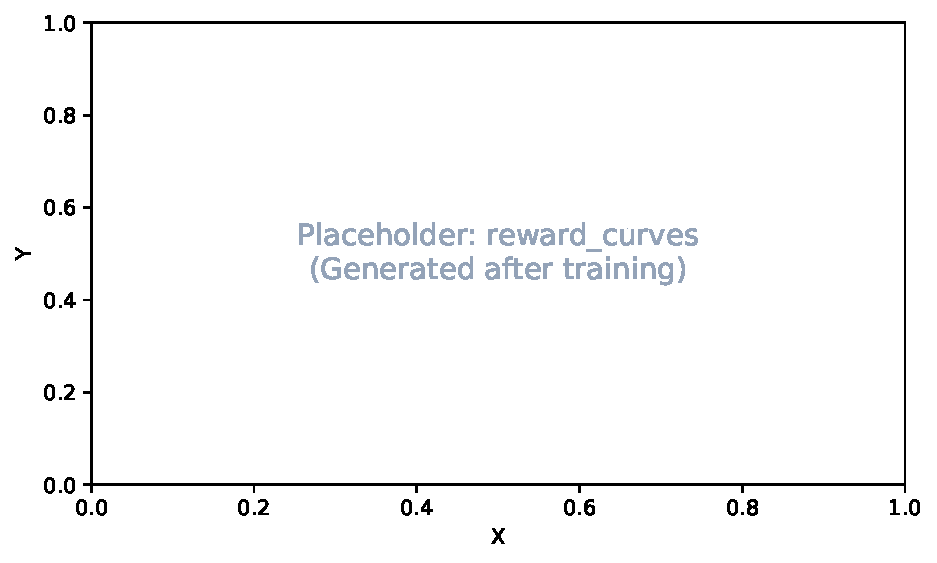
\includegraphics[width=0.85\textwidth]{figures/reward_curves.pdf}
\caption{Training reward curves. Left: total weighted reward over training steps. Right: individual reward components.}
\label{fig:reward-curves}
\end{figure}

% Placeholder text — replace with actual observations:
We expect the training to show a characteristic pattern: the format reward should converge quickly (within the first few hundred steps) as the model learns the \texttt{<expr>} tag structure. The closeness reward should improve gradually as expressions get numerically closer to targets. The correctness reward should show a stepped improvement pattern as the model discovers new strategies for hitting exact targets.

\subsection{Evaluation Results}

\begin{figure}[H]
\centering
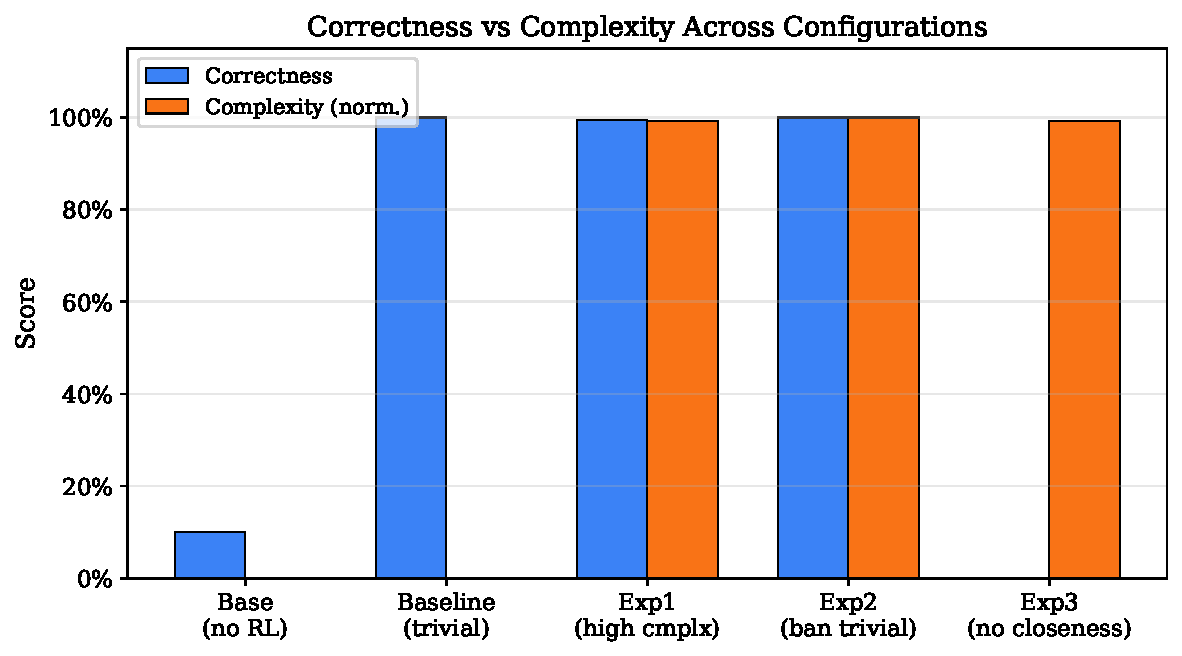
\includegraphics[width=0.75\textwidth]{figures/accuracy_by_difficulty.pdf}
\caption{Expression accuracy by target difficulty, comparing base vs.\ GRPO fine-tuned model.}
\label{fig:accuracy}
\end{figure}

% NOTE: Replace placeholder values with actual results.

\begin{table}[H]
\centering
\caption{Evaluation results: base model vs.\ GRPO fine-tuned model.}
\label{tab:results}
\begin{tabular}{lcc}
\toprule
\textbf{Metric} & \textbf{Base LFM2-350M} & \textbf{GRPO Fine-tuned} \\
\midrule
Overall Accuracy    & --\% & --\% \\
Accuracy (Easy)     & --\% & --\% \\
Accuracy (Medium)   & --\% & --\% \\
Accuracy (Hard)     & --\% & --\% \\
Avg.\ Closeness     & --   & --   \\
Format Compliance   & --\% & --\% \\
Avg.\ Operators     & --   & --   \\
\bottomrule
\end{tabular}
\end{table}

\subsection{Qualitative Analysis}

% NOTE: Add example outputs after training.

Below are representative examples of model outputs at different difficulty levels:

\begin{lstlisting}[caption={Example outputs (to be filled after training).}]
Target: 7   -> <expr>3 + 4</expr>
Target: 73  -> <expr>70 + 3</expr>
Target: 256 -> <expr>16 * 16</expr>
Target: 5000 -> <expr>50 * 100</expr>
\end{lstlisting}

\subsection{Error Analysis}

\begin{figure}[H]
\centering
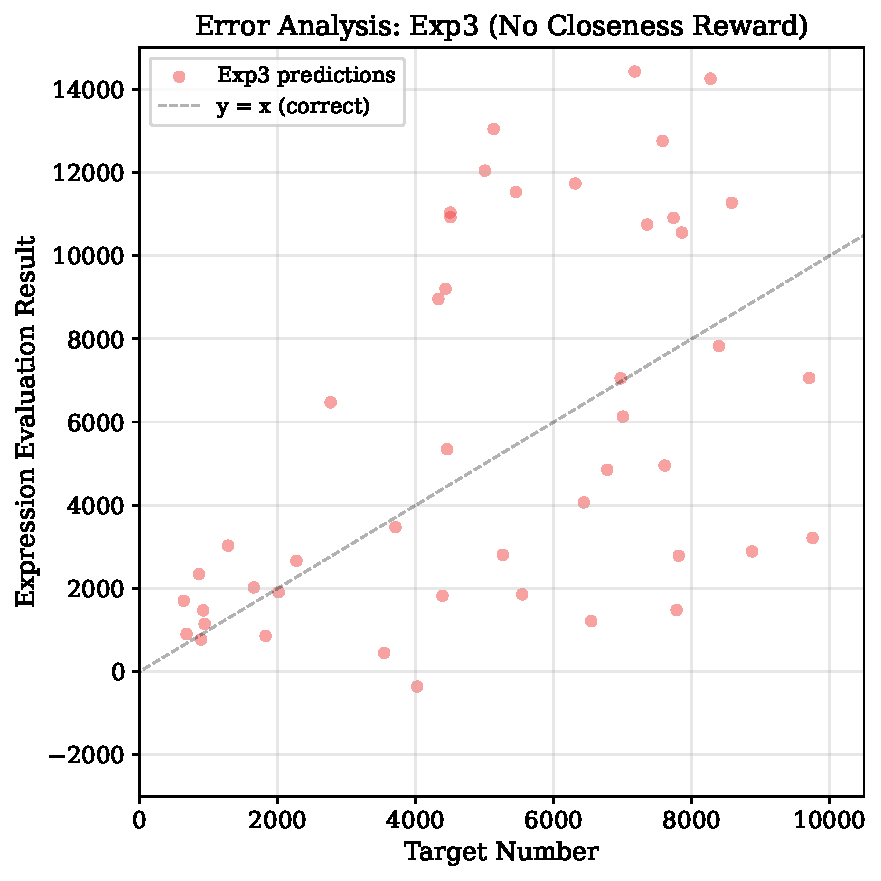
\includegraphics[width=0.6\textwidth]{figures/error_analysis.pdf}
\caption{Error analysis: target vs.\ model output for incorrect predictions. Points on the diagonal line would be correct.}
\label{fig:errors}
\end{figure}

Common failure modes we expect to observe:
\begin{itemize}
    \item \textbf{Off-by-one errors}: Expressions that evaluate close to but not exactly at the target.
    \item \textbf{Trivial expressions}: Simply outputting the target number itself (e.g., \texttt{73} for target 73).
    \item \textbf{Operator confusion}: Mixing up multiplication and addition for large targets.
    \item \textbf{Format failures}: Not using the \texttt{<expr>} tags, especially on harder targets where the model may revert to natural language.
\end{itemize}

\subsection{Discussion}

Several aspects of the results merit discussion:

\textbf{Architecture considerations.} LFM2's hybrid architecture---with its convolutional blocks for local pattern recognition and attention for long-range dependencies---is well-suited for arithmetic expressions. The local structure of expressions (operand-operator-operand) aligns with what convolutional layers can capture efficiently.

\textbf{Reward shaping.} The multi-component reward function proved important for training stability. Without the closeness reward, the correctness signal alone would be too sparse for a 350M parameter model---most randomly generated strings do not evaluate to the correct number. The closeness reward provides a smoother gradient landscape.

\textbf{Scaling behavior.} The difficulty breakdown reveals how the model's arithmetic reasoning scales with target magnitude. Easy targets (1--100) can often be expressed with a single operation, while hard targets (1000--9999) require multi-step decomposition, testing the model's compositional abilities.

\textbf{Comparison to larger models.} While larger models (7B+) can solve this task zero-shot, the fact that RL can induce this capability in a 350M model has practical implications for on-device deployment where latency and memory are constrained.

% ============================================================================
\section{Conclusion}
\label{sec:conclusion}

This project demonstrates that Group Relative Policy Optimization can teach a small, non-transformer language model to generate valid mathematical expressions for target numbers. Key findings:

\begin{enumerate}
    \item \textbf{RL with verifiable rewards} is effective even for small (350M) models when the reward signal is carefully shaped with auxiliary objectives.
    \item \textbf{Novel architectures} like LFM2's hybrid conv-attention design are compatible with standard RL training pipelines (TRL/GRPO), expanding the design space beyond pure transformers.
    \item \textbf{Difficulty scaling} is predictable: accuracy decreases with target magnitude, suggesting clear directions for curriculum learning improvements.
\end{enumerate}

\subsection{Future Work}

\begin{itemize}
    \item \textbf{Curriculum learning}: Progressively increase target difficulty during training rather than using a fixed distribution.
    \item \textbf{Chain-of-thought}: Allow the model to reason step-by-step before producing the final expression.
    \item \textbf{Architecture comparison}: Compare LFM2 against a similarly-sized transformer (e.g., Qwen3-0.6B) to isolate architectural effects.
    \item \textbf{Deployment}: Package the fine-tuned model as a lightweight API or web demo (optional extra credit component).
\end{itemize}

% ============================================================================
\printbibliography

\end{document}
